\documentclass[12pt]{article}


\usepackage{amssymb}
\usepackage{amsmath}
\usepackage{fullpage}
\usepackage{epsfig}
\usepackage{epstopdf}
\everymath{\displaystyle}

\newif\ifans

\ansfalse

\begin{document}

\begin{center}
\underline{\LARGE{Chapter 1.6 Practice Problems}}
\end{center}

\noindent EXPECTED SKILLS:

\begin{itemize}

\item Know where the trigonometric and inverse trigonometric functions are continuous.

\item Be able to use $\lim_{x\rightarrow0}\frac{\sin{x}}{x}=1$ or $\lim_{x \rightarrow 0}\frac{1-\cos{x}}{x}=0$ to help find the limits of functions involving trigonometric expressions, when appropriate.

\item Understand the squeeze theorem and be able to use it to compute certain limits.

\end{itemize}

\noindent PRACTICE PROBLEMS:

\medskip

\noindent {\bf Evaluate the following limits.  If a limit does not exist, write DNE, $+\infty$, or $-\infty$ (whichever is most appropriate).}

\begin{enumerate}

\item  $\displaystyle \lim_{x\rightarrow \frac{\pi}{4}} \sin{(2x)}$ 

\ifans{\fbox{1}} \fi

\item $\displaystyle \lim_{\theta \rightarrow \pi}{(\theta \cos{\theta})}$

\ifans{\fbox{$-\pi$}} \fi

\item  $\displaystyle \lim_{x\rightarrow 0^+} \csc x$ 

\ifans{\fbox{$+\infty$}} \fi

\item  $\displaystyle \lim_{x\rightarrow \frac{\pi}{2}^+} \tan x$ 

\ifans{\fbox{$-\infty$}} \fi

\item  $\displaystyle \lim_{x\rightarrow \frac{\pi}{2}^-} \tan x$ 

\ifans{\fbox{$+\infty$}} \fi

\item $\displaystyle \lim_{x \rightarrow \frac{\pi}{4}}{\sec{x}}$

\ifans{\fbox{$\sqrt{2}$}} \fi

\item $\displaystyle \lim_{x\rightarrow 0}{\left(\frac{\sin{x}}{3x}\right)}$ 

\ifans{\fbox{$\displaystyle \frac{1}{3}$}} \fi

\item $\displaystyle \lim_{x\rightarrow 0}{\left(\frac{\sin{3x}}{3x}\right)}$ 

\ifans{\fbox{$\displaystyle 1$}} \fi

\item $\displaystyle \lim_{x\rightarrow 0}{\left(\frac{\sin{x}}{|x|}\right)}$

\ifans{\fbox{DNE}} \fi

\item $\displaystyle \lim_{x\rightarrow 0}{\left(\frac{1-\cos{x}}{4x}\right)}$

\ifans{\fbox{$0$}} \fi

\item $\displaystyle \lim_{x\rightarrow 0^-}{\left(\frac{\cos x}{x}\right)}$ 

\ifans{\fbox{$-\infty$}} \fi

\item $\displaystyle \lim_{x\rightarrow 0}{\left(\frac{\sin 2x}{x}\right)}$

\ifans{\fbox{2}} \fi

\item $\displaystyle \lim_{x\rightarrow 0}{\left(\frac{\tan 2x}{x}\right)}$

\ifans{\fbox{2}} \fi

\item $\displaystyle \lim_{x\rightarrow 0}{\left(\frac{1-3\cos{x}}{3x}\right)}$

\ifans{\fbox{DNE}} \fi

\item $\displaystyle \lim_{x\rightarrow \infty}{\arccos{\left(\frac{-x^2}{x^2+3x}\right)}}$ 

\ifans{\fbox{$\displaystyle \pi$}} \fi

\item $\displaystyle \lim_{x\rightarrow 0}{\left(\frac{3x^2}{1-\cos^2{x}}\right)}$

\ifans{\fbox{3}} \fi

\item $\displaystyle \lim_{x \rightarrow 0}{\left(\frac{\tan{5x}}{\sin{9x}}\right)}$

\ifans{\fbox{$\displaystyle \frac{5}{9}$}} \fi

\item {\bf Multiple Choice:} Evaluate $\lim_{x \rightarrow 0} \frac{\tan^2{x}}{x^2}$

\begin{enumerate}

\item $-1$

\item 0

\item 1

\item $-\infty$

\item $+\infty$

\end{enumerate}

\ifans{\fbox{c}} \fi

\end{enumerate}

\noindent {\bf For problems 19-23, evaluate the following limits by first making an appropriate substition.  If the limit does not exist, write DNE, $+\infty$, or $-\infty$ (whichever is most appropriate).}

\begin{enumerate}
\setcounter{enumi}{18}

\item $\displaystyle \lim_{x\rightarrow \infty}{\left(e^x \sin {(e^{-x})}\right)}$\\

\ifans{\fbox{1}} \fi

\item $\displaystyle \lim_{x\rightarrow 1}{\left(\frac{\sin{(\ln x^5)}}{\ln x}\right)}$ 

\ifans{\fbox{5}} \fi

\item $\displaystyle \lim_{x \rightarrow \frac{\pi}{2}^+}{e^{\sec{x}}}$

\ifans{\fbox{0}} \fi

\item $\displaystyle \lim_{x \rightarrow 0}{\sin{\left(\frac{1}{x^2}\right)}}$

\ifans{\fbox{DNE}} \fi

\item $\displaystyle \lim_{x \rightarrow 0^+}{\tan^{-1}{(\ln{x})}}$

\ifans{\fbox{$\displaystyle -\frac{\pi}{2}$}} \fi

\end{enumerate}

\noindent {\bf For problem 24-28, determine the value(s) of $x$ where the given function is continuous.} 

\begin{enumerate}
\setcounter{enumi}{23}

\item $f(x) = \csc{x}$ 

\ifans{\fbox{$f(x)$ is continuous for all $x \neq \pi k$, where $k$ is any integer.}} \fi

\item $f(x) = e^{\sin {x}}$

\ifans{\fbox{$f(x)$ is always continuous.}} \fi

\item $\displaystyle f(x) = \frac{1}{1-2\cos{x}}$ on $[0,2\pi]$ 

\ifans{\fbox{$f(x)$ is continuous for all $x$ in $[0,2\pi]$ except for $\displaystyle x=\frac{\pi}{3}$ and $\displaystyle x=\frac{5\pi}{3}$}} \fi

\item $f(x) = \sin^{-1}{x}$ 

\ifans{\fbox{$f(x)$ is continuous on its domain of $[-1,1]$}} \fi

\item $\displaystyle f(x)=\left\{
\begin{array}{lll}
\cos{x} & \text{if} & x< \frac{\pi}{4}\\
&\\
\sin{x} & \text{if} & x\geq \frac{\pi}{4}
\end{array}\right.$

\ifans{\fbox{$f(x)$ is always continuous.}} \fi

\item Find all non-zero value(s) of $k$ so that $\displaystyle f(x)=\left\{\begin{array}{lll}
\frac{3\sin{(kx)}}{x} & \text{if} & x>0\\
&&\\
6k^2+5x & \text{if} & x \leq 0
\end{array}\right.$
is continuous at $x=0$.

\ifans{\fbox{$\displaystyle k=\frac{1}{2}$}} \fi

\item Use the Intermediate Value Theorem to prove that there is at least one solution to $\cos{x}=x^2$ in $(0,1)$.

\ifans{\fbox{\parbox{1\linewidth}{Let $f(x)=\cos{(x)}-x^2$.  Since $f(x)$ is continuous on $(-\infty,\infty)$, it is also continuous on $[0,1]$.  Notice that $f(0)=1>0$ and $f(1)=\cos{(1)}-1<0$.  Thus, the Intermediate Value Theorem states that there must be some $c$ in $(0,1)$ such that $f(c)=0$.  i.e., there must be at least one $c$ in $(0,1)$ such that $\cos(c)-c^2=0$ $\implies$ $\cos{(c)}=c^2$, as desired.}}} \fi

\item Let $f(x)$ be a function which satisfies $\displaystyle 5x-6 \leq f(x) \leq x^2+3x-5$ for all $x \geq 0$.  Compute $\displaystyle \lim_{x \rightarrow 1}{f(x)}$.

\ifans{\fbox{$-1$}} \fi

\item The graph of $\displaystyle f(x)=x^2e^{\cos{(1/x)}}$ is shown below on $[-0.1,0.1]$:\\

\begin{center}
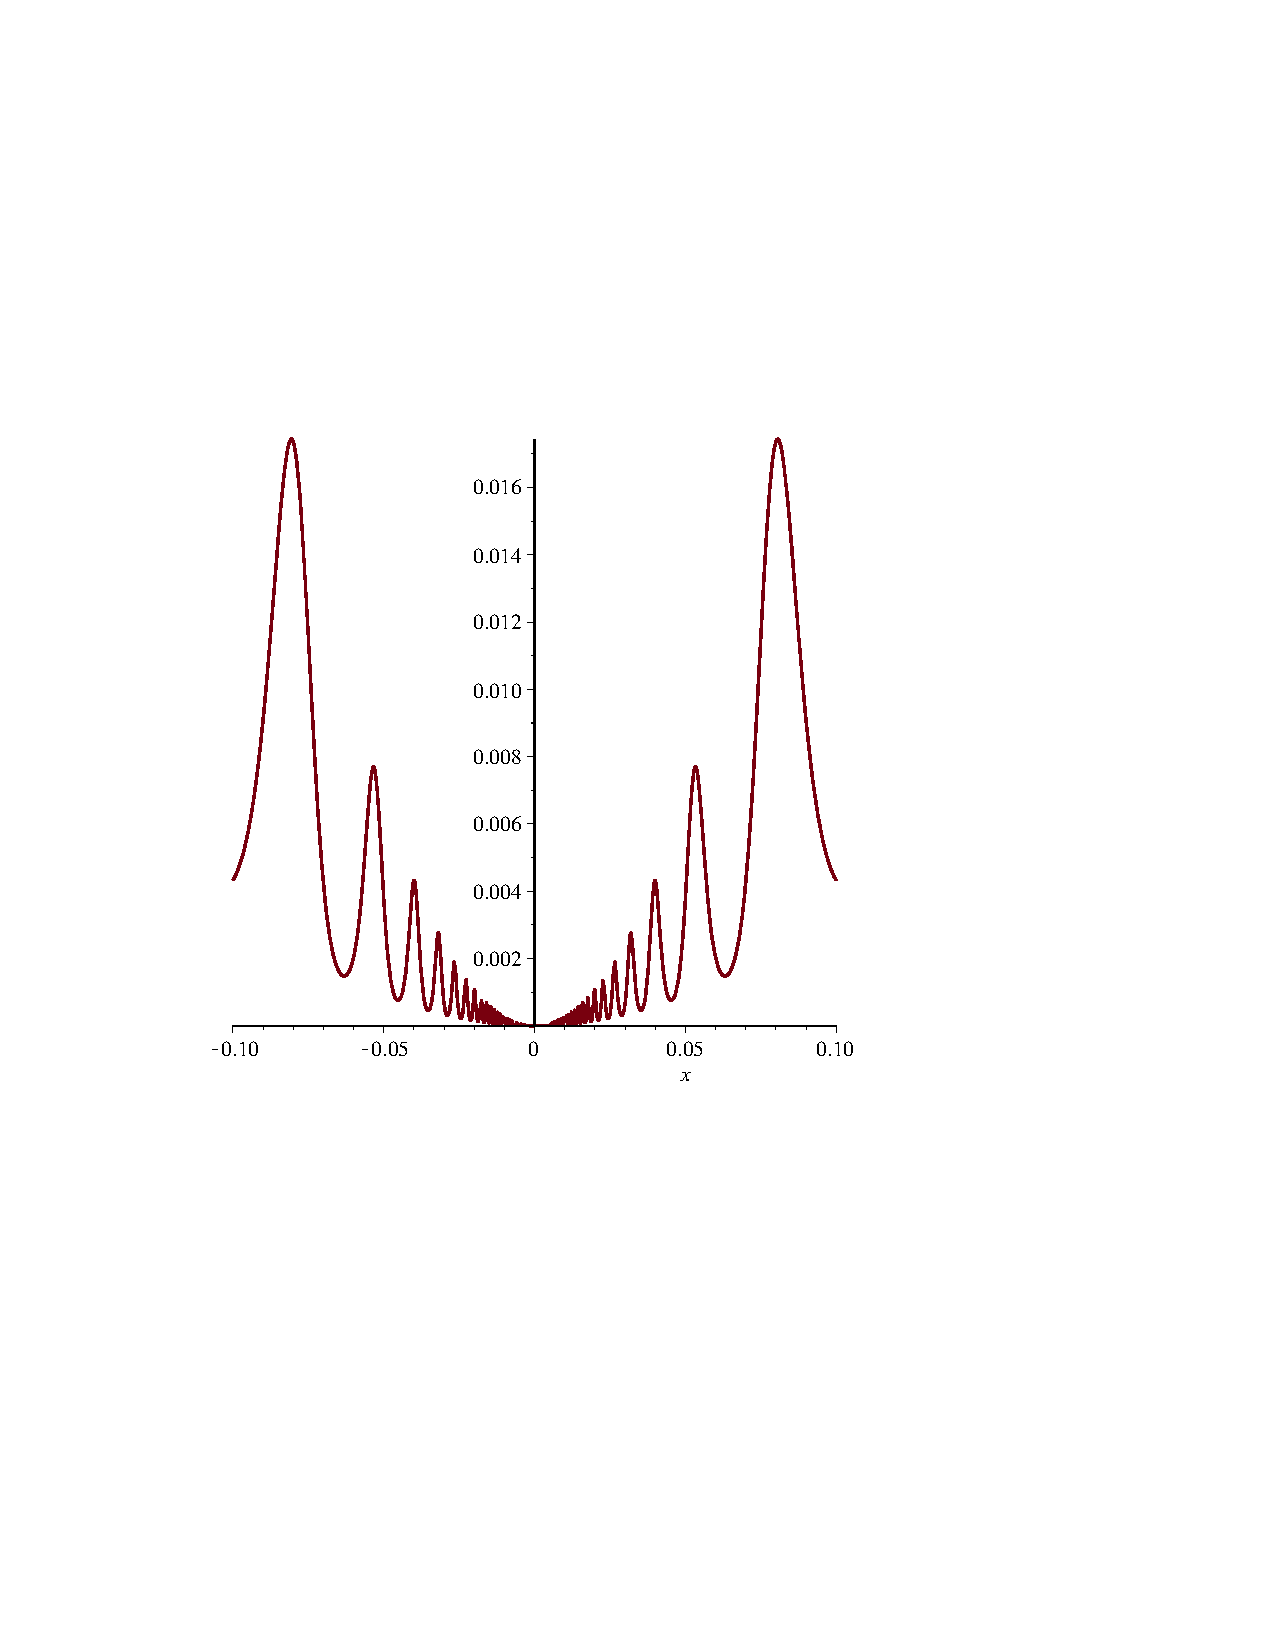
\includegraphics[scale=.6]{squeezegraph.pdf}
\end{center}

Make a conjecture about $\displaystyle \lim_{x \rightarrow 0}{f(x)}$ and then use the Squeeze Theorem to show this is true.

\ifans{\fbox{\parbox{1\linewidth}{Claim: $\displaystyle \lim_{x\rightarrow 0}{f(x)}=0$\\
Proof: We can bound $\displaystyle f(x)=x^2e^{\cos{(1/x)}}$ above by $ex^2$ and below by $e^{-1}x^2$, both of which approach 0 as $x$ approaches 0.  Thus, by the squeeze theorem, $f(x) \rightarrow 0$ as well when $x \rightarrow 0$.}}} \fi

\item Let $x$ be a fixed real number.  Compute $\lim_{h \rightarrow 0}\frac{\sin{(x+h)}-\sin{x}}{h}$.  (Hint: The identity $\sin{(A+B)}=\sin{A}\cos{B}+\cos{A}\sin{B}$ will be useful.)

\ifans{\fbox{$\cos{x}$}} \fi

\end{enumerate}

\end{document}